%% Full length research paper template
%% Created by Simon Hengchen and Nilo Pedrazzini for the Journal of Open Humanities Data (https://openhumanitiesdata.metajnl.com)

\documentclass{article}
\usepackage[english]{babel}
\usepackage[utf8]{inputenc}
\usepackage{johd}
\graphicspath{ {./images/} }

\title{Annotation Guidlines for Explainability Annotations for Legal Judgment Prediction in Switzerland}

\author{Nina Baumgartner}

\date{} %leave blank
\begin{document}

\maketitle
\section{Introduction}
\subsection{Annotation Goal}
Recently  \citet{Niklaus_2021} presented a dataset for legal Judgment prediction including 85k Swiss Federal Supreme Court decisions. Using Hierarchical BERT they achieved a Macro-F1 Score of approximately 68-70\%. Nevertheless, the inner workings of such models are still mostly unknown and the results thus not interpretable. 
For this reason, this annotation task focuses on the explainability of these predictions. With your annotation you will give your insight as a legal expert and tag parts of the facts that support or oppose the judgment. 
These guidelines are based on the work of \cite{Reiter+2020+193+202}, \cite{Leitner_2019} and \cite{pustejovsky2012natural}. They are a work-in-progress in collaboration with Lynn Grau, Angela Stefanelli and Thomas Lüthi.

\subsection{Dataset}
For this task a subset of the Swiss court ruling corpus presented by \cite{Niklaus_2021} containing 108 cases was created. In most of these cases the model worked well and indicated the correct judgment form the facts given to it. The 108 cases are equally distributed among the three languages German, French and Italian. Each language set contains six cases over six years. With each year having two cases per legal area\footnote{The chosen legal areas are categorized as penal law, social law and civil law}: One with the verdict approved and one with the verdict dismissed.

\subsection{Disclaimer}
This document is a work-in-progress. If you have questions or find any errors in these instructions while doing the annotation please feel free to contact the maintainer. Please help with collecting examples to complete these guidelines.

\section{Annotation Entities}
Although you will only be annotating the fact section of a ruling, you will have access to the full document (via a link on Prodigy) and the judgment will be clearly indicated on the prodigy interface. You can and should use these other resources as an indicator on which part of the facts are of greatest importance.
\subsection{Sentences and Sub-Sentences}
The annotation will focus on the sentences and sub-sentences. For this task we define a sentence as a self-contained linguistic unit consisting of multiple words, terminated with a period, semicolon, colon, question mark or exclamation mark. A entire sentence is the largest entity to be annotated. A sentence can consist of multiple sub-sentences usually separated with a "and" or a comma. It is possible that a sentence contains two sub-sentences opposing each other, which should be consequently annotated with different labels. These sub-sentences are the smallest units that should be annotated. We hope that by choosing this scope it is possible to indicate what the different parts of the sentences denote in the context of the judgment and to subsequently better explain the decisions of the model.

\subsection{Lower Court}
In addition to sentences you will also have to annotate the last lower court of each case. As seen in Figure \ref{rubrum} the Rubrum of the ruling indicates the last lower court. The last lower court is composed of the name of the court e.g. "Verwaltungsgericht" and the location "Kanton Luzern".

\begin{figure}[h]
    \makebox[\textwidth]{\fbox{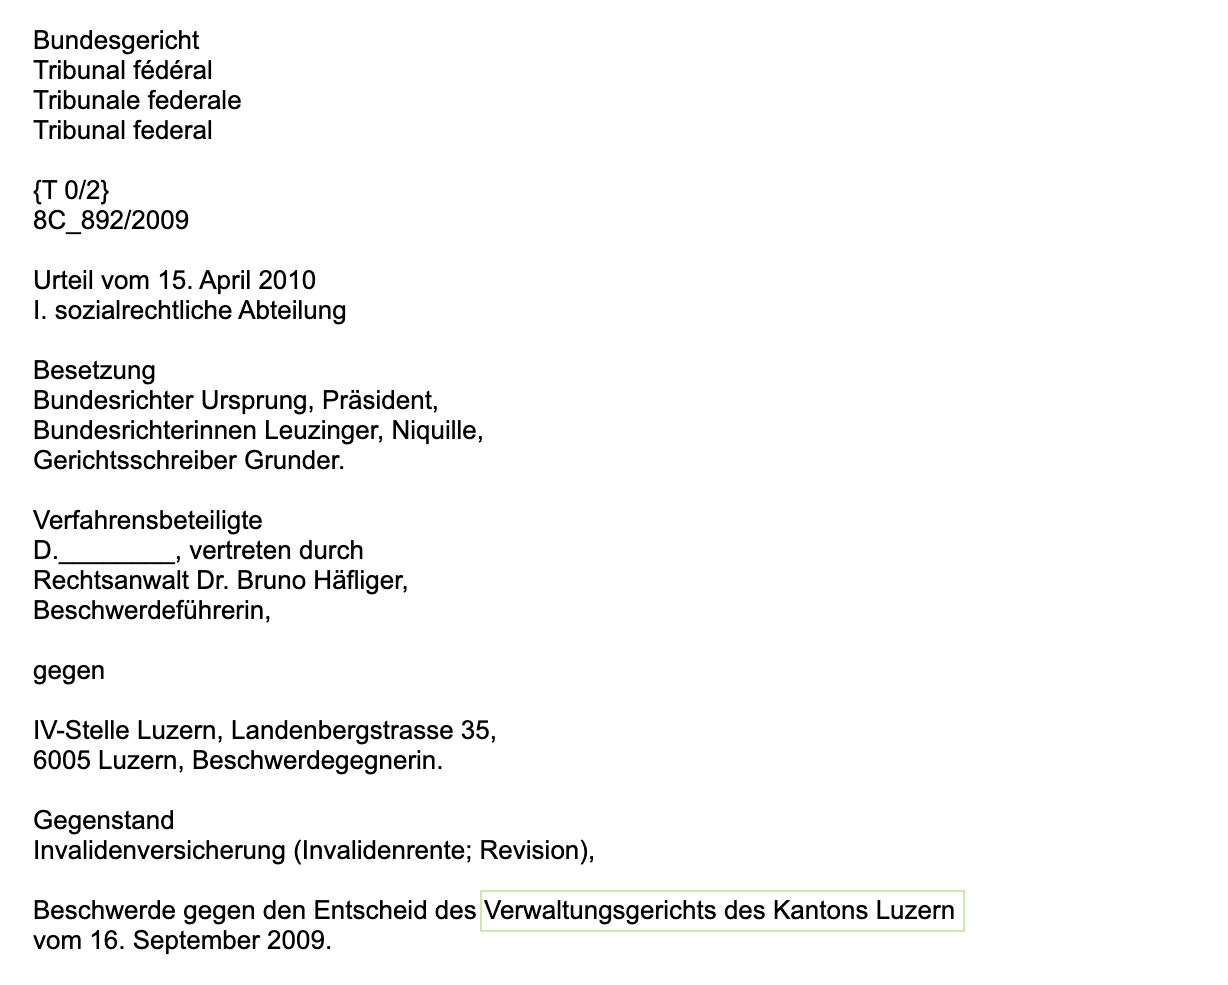
\includegraphics[width=\textwidth]{Bachelorthesis/Annotationguidelines/images/rubrum_8C_892-2009.png}}}
     \caption{Example of a Rubrum with the lower court highlighted.
     Judgment (of the Federal Court) 8C-892/2009 form April 15th 2010}
     \label{rubrum}
\end{figure}
\pagebreak

\section{Annotation Categories}
To annotate the sentences of each fact section you will be using two labels,  \emph{Supports judgment} and \emph{Opposes verdict}. You should also highlight the lower court for each judgement. In addition, you will be given several options for dealing with problematic cases, which should help to improve the dataset, these guidelines and the annotations themselves.

\subsection{Supports Judgment}
This label is used when a sentence or sub-sentence supports the judgment. Every sub-sentence that supports the judgment should be annotated.
@ToDo Example and more explanation

\subsection{Opposes Judgment}
This label is used when a sentence or sub-sentence opposes the judgment. Every sub-sentence that opposes the judgment should be annotated.
@ToDo Example and more explanation

\subsection{Lower Court}
This label is used to highlight the last lower court of the case. To label the last lower court highlight the name and the location of the court  as one instance (see Figure \ref{lower-court}).
\begin{figure}[h]
    \makebox[\textwidth]{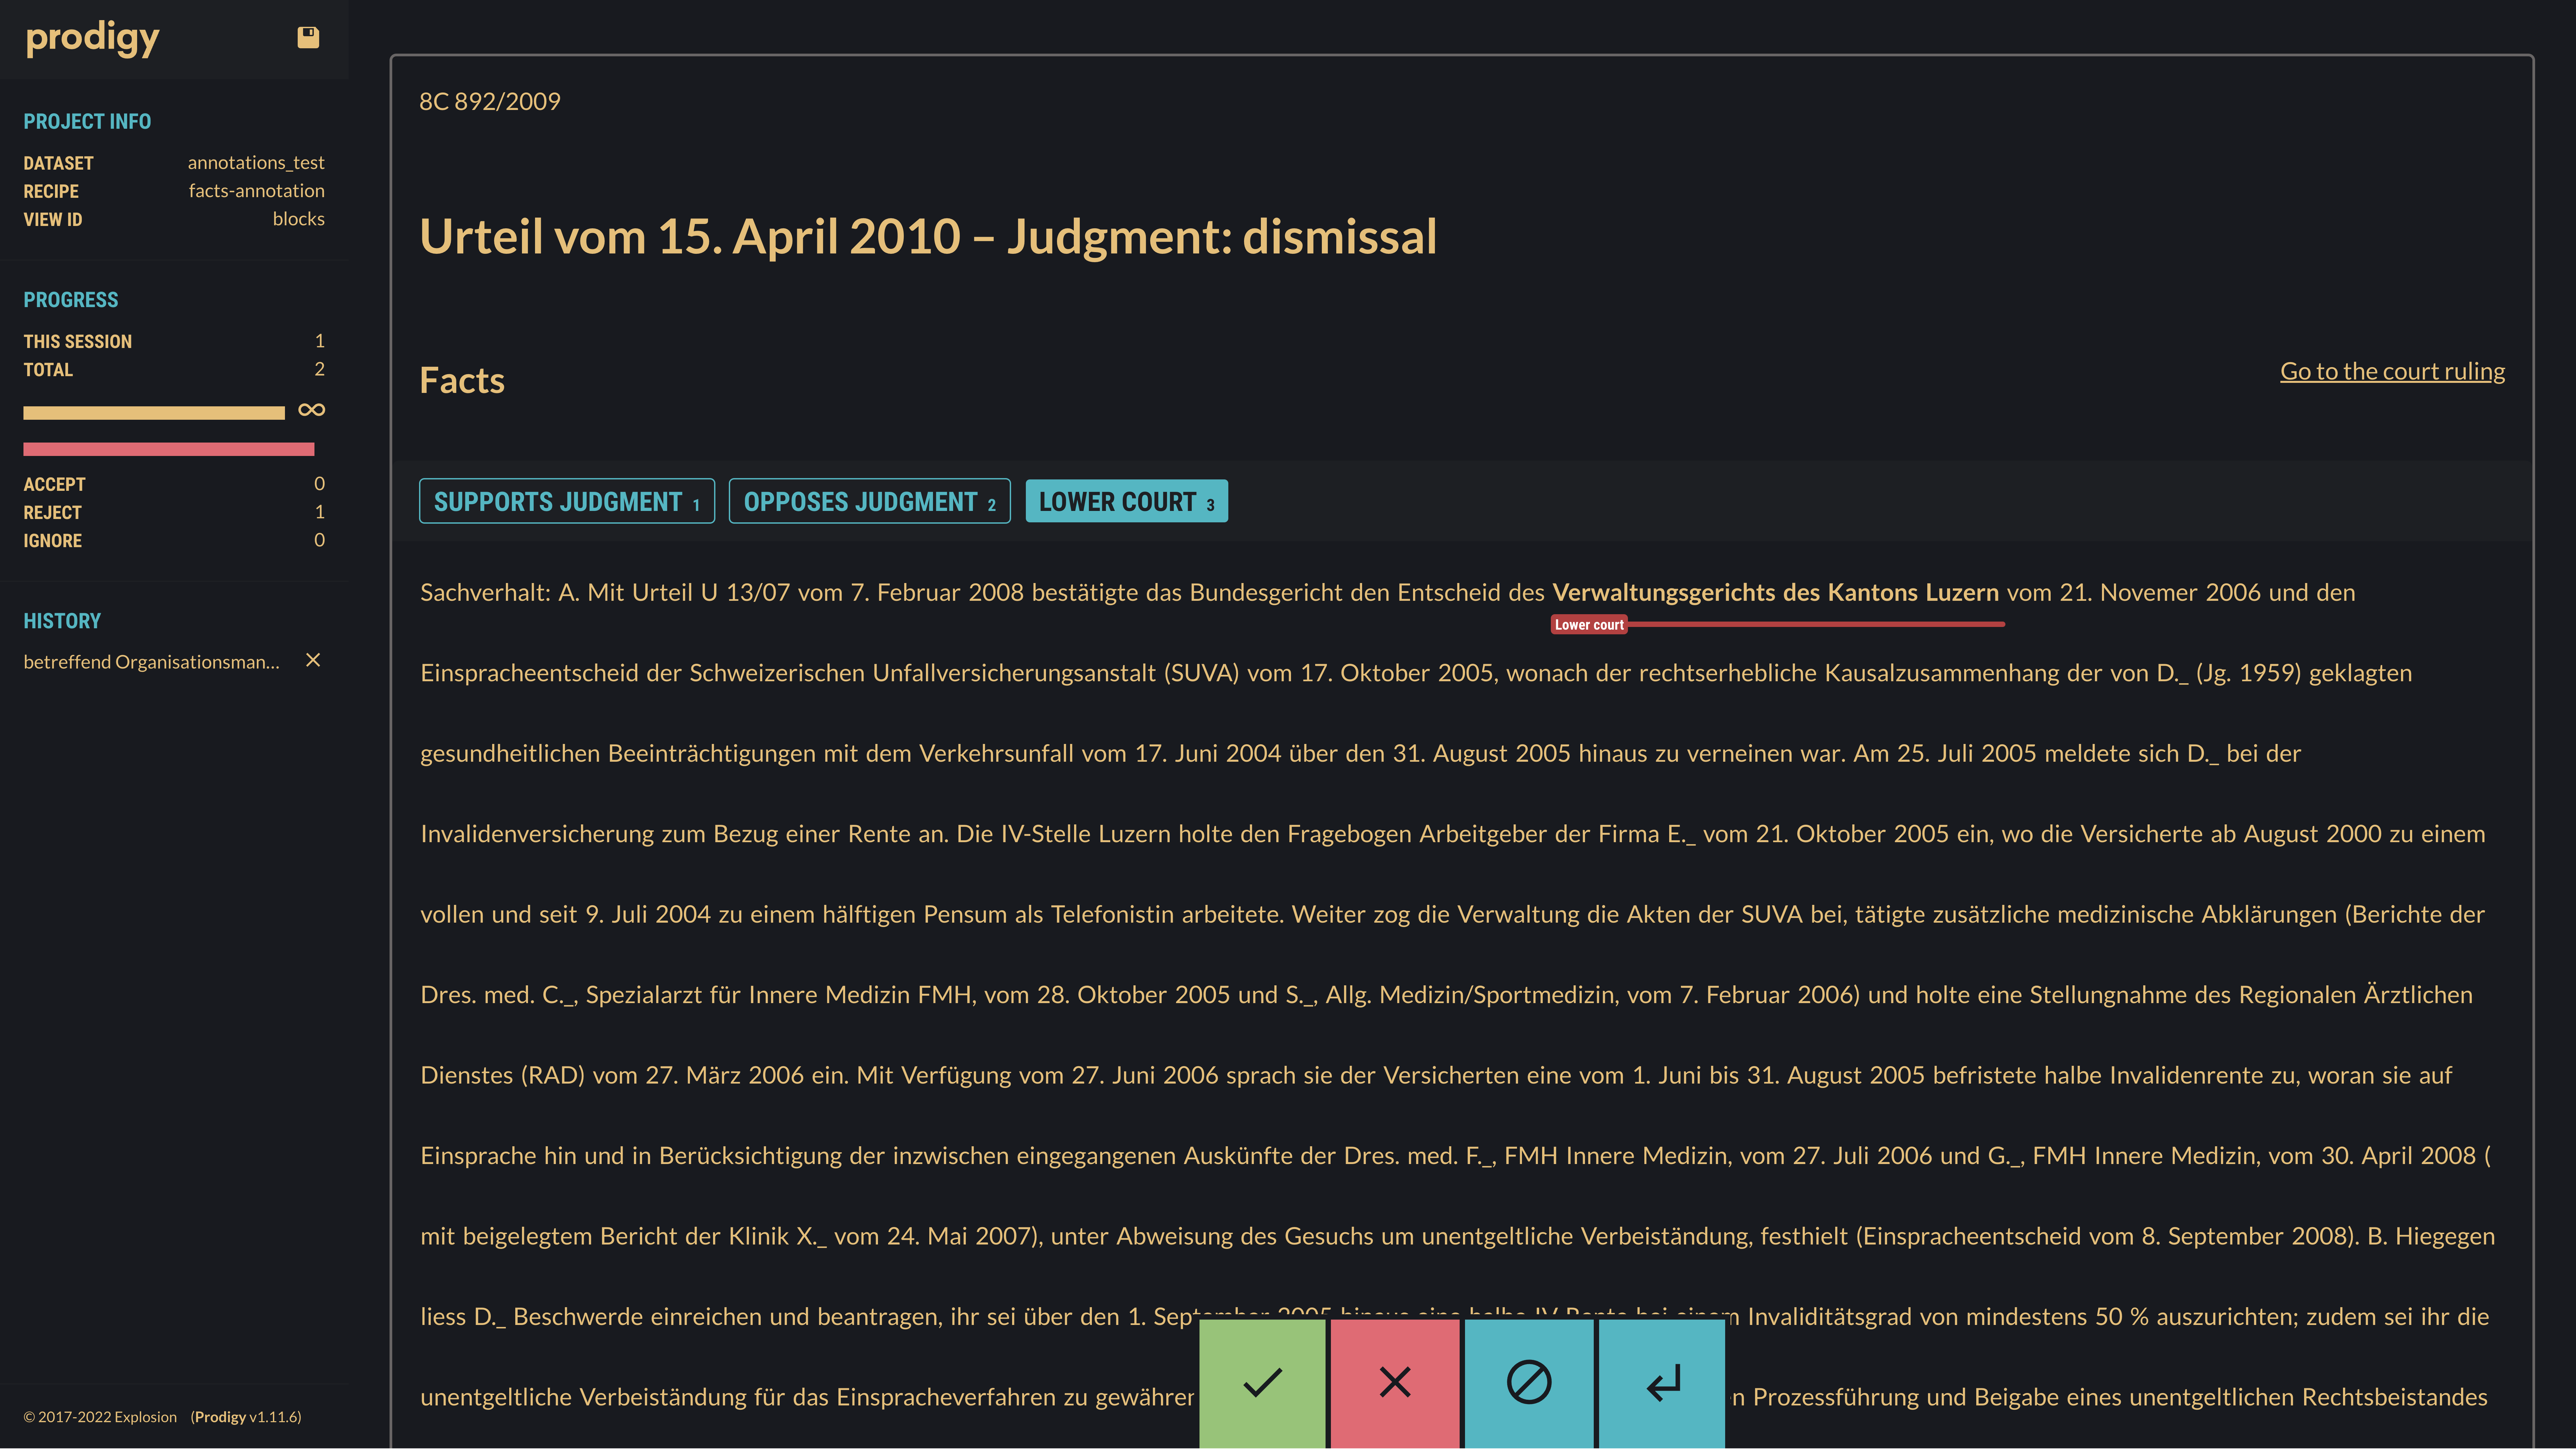
\includegraphics[width=\textwidth]{Bachelorthesis/Annotationguidelines/images/prodigy-lower-court.png}}
     \caption{Example of a highlighted lower court in Prodigy.}
     \label{lower-court}
\end{figure}
\pagebreak

\subsection{Neutral}
Every not-labeled sub-sentence is considered neutral. This is not a label per se but merely how the system interprets words or sentences which are not assigned one of the labels above. It is important for the analysis that even the neutral sentences are annotated which in our case means to omit them.

One example in German of an neutral expression which should not be tagged with a label is the word \emph{"Sachverhalt:"}. This word only indicates the beginning of the fact section and should be left out as a neutral part of the facts because it does not give us any further information on the explainability of the judgment. 

\subsection{Problematic Cases}
Problematic cases can occur because this annotation task is an iterative process. For now, we differentiate between three possible types of such cases.

\subsubsection{Rejected Cases}
If a case is badly tokenized\footnote{Tokenized means that the system did not properly separate the words.} or there is another formal error it should be rejected. Please state your reasoning in the comment window using the comment pattern below and reference the \nameref{reject-ignore-case} section of this document for the details on how to properly reject a case. Figure \ref{reject_case} is an example of a case with formal errors. 
\begin{figure}[h!]
    \makebox[\textwidth]{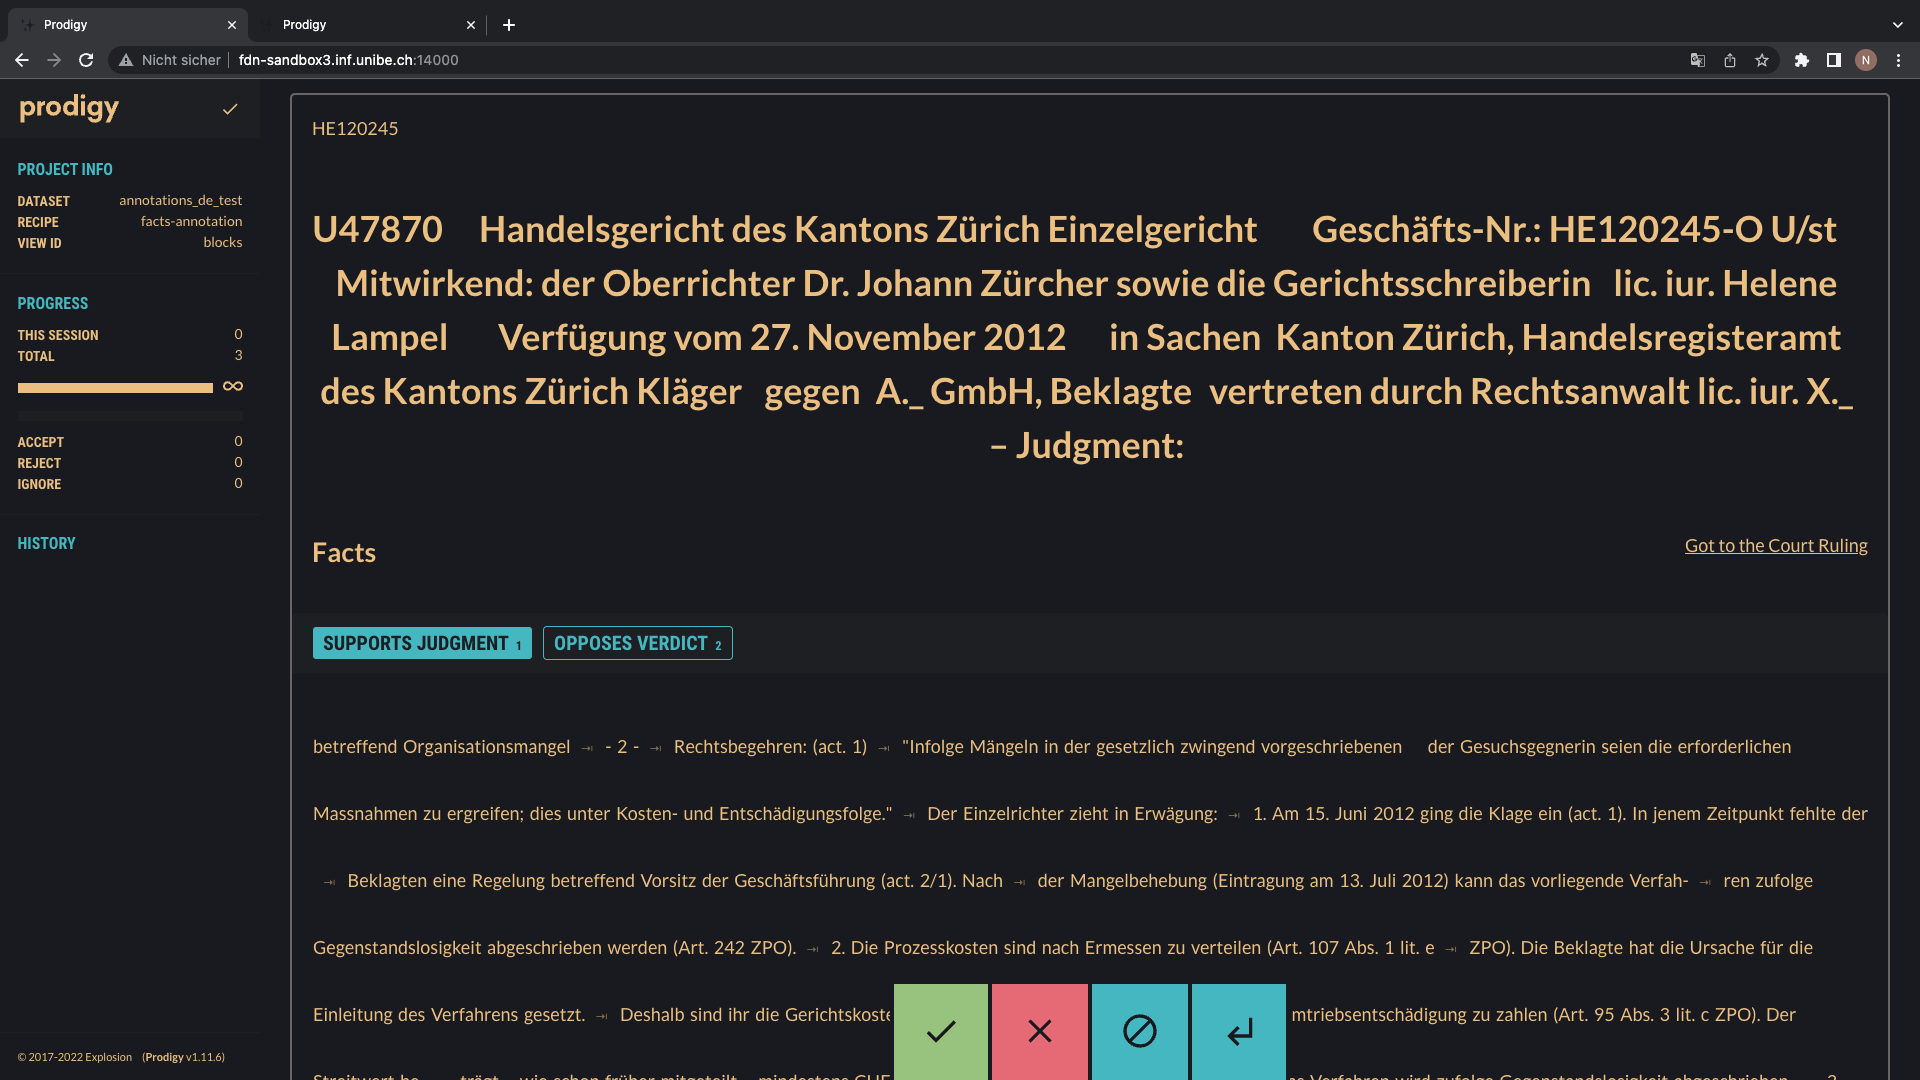
\includegraphics[width=\textwidth]{Bachelorthesis/Annotationguidelines/images/reject_case.png}}
     \caption{Example of a case containing a formal error which should be rejected. Here the title was parsed incorrectly, the judgment is missing and the facts are tokenized wrongly and incomplete.}
     \label{reject_case}
\end{figure}

\subsubsection{Ignored Cases}
If a case is to short or otherwise unfit for the annotation it should be ignored. To ignore it please state your reasoning in the comment section and follow the steps explained in the \nameref{reject-ignore-case} section of this document below. 

\subsubsection{Other Problematic Cases}
There might be cases without formal errors where you have difficulties to annotate (neither reject nor ignore). In such cases, please annotate to the best of your ability and explain your reasoning in the comment section.

\subsubsection{Comment Structure}
\begin{mdframed}[frametitle={Comment for rejecting and ignoring case}]
\emph{Number of case – Annotators name}

\begin{itemize}
	\item Why did you ignore/reject this case?
\end{itemize}	
\end{mdframed}

\begin{mdframed}[frametitle={Comment for generally problematic case}]
\emph{Number of case – Annotators name}

\begin{itemize}
	\item Why is this case problematic and difficult to annotate?

\item How did you decide on your annotation?
\end{itemize}
\end{mdframed}

\section{Implementation: How to Annotate the Dataset Using Prodigy}
This section explains how to use the annotation tool Prodigy\footnote{\href{https://prodi.gy/}{https://prodi.gy/}}. We built a custom recipe for this task which lets you annotate the facts section of a given court decision.

\subsection{Access}
The Prodigy instance can only be accessed via the University of Bern network. If you want to annotate from home you must use the VPN of the University of Bern\footnote{\href{https://serviceportal.unibe.ch/sp?id=kb_article_view&sys_kb_id=00cb11e51b005050134ddc6a9b4bcb49}{https://serviceportal.unibe.ch/sp?id=kb_article_view&sys_kb_id=00cb11e51b005050134ddc6a9b4bcb49}}.
If you are connected to the university network you can access Prodigy via one of the following URLs:
\begin{itemize}
\item German case annotations:
\begin{itemize}
\item Angela: \href{http://fdn-sandbox3.inf.unibe.ch:11000/?session=angela}{http://fdn-sandbox3.inf.unibe.ch:11000/?session=angela}
    \item Lynn: \href{http://fdn-sandbox3.inf.unibe.ch:11000/?session=lynn}{http://fdn-sandbox3.inf.unibe.ch:11000/?session=lynn}
    \item Thomas: \href{http://fdn-sandbox3.inf.unibe.ch:11000/?session=thomas}{http://fdn-sandbox3.inf.unibe.ch:11000/?session=thomas}
\end{itemize}
    \item French case annotations: \href{http://fdn-sandbox3.inf.unibe.ch:12000/}{http://fdn-sandbox3.inf.unibe.ch:12000/}
    \item Italian case annotations: \href{http://fdn-sandbox3.inf.unibe.ch:13000/}{http://fdn-sandbox3.inf.unibe.ch:13000/}
\end{itemize}

Before you can start you will be asked to provide a \emph{username} and a \emph{password}, which will be give to you by the maintainer of the annotation process. After the login procedure you should now see an overview of the case and you can start with your annotation.

\subsection{Annotate a Sub-Sentence}
To label a phrase with a tag, highlight it with your cursor and choose the corresponding label. To delete a tag simply click on the tagged words again. As seen in Figure \ref{sentence_annotation} the two label appear in two different colors. By hovering over an annotated section the delete toggle appears.

\begin{figure}[h]
    \makebox[\textwidth]{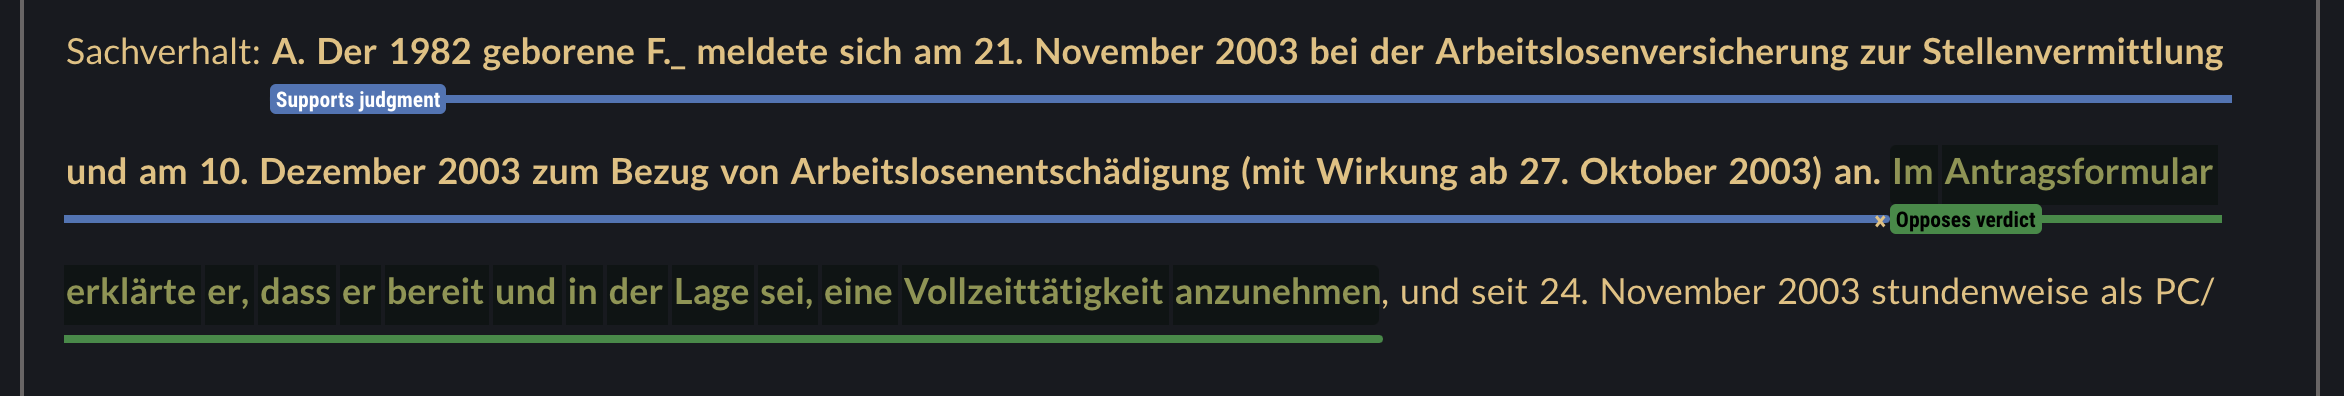
\includegraphics[width=\textwidth]{Bachelorthesis/Annotationguidelines/images/sentence_annotation.png}}
     \caption{Screenshot of sentence labeling in prodigy.}
     \label{sentence_annotation}
\end{figure}


If you are happy with your annotation you can accept it by clicking on the green check labeled with [1] in Figure \ref{overview} and save it by pressing the save button in the left corner referenced by the number [2].
To see your progress you can look at the information displayed on the left (see number [3] on Figure \ref{overview}). If you want to access the original document you can click on the link in the right corner (see number [4]). Please do not forget to safe your progress using the save button [2].

If you want to skip a case, because you already annotated it. Please use the accept button [1] to get to the next case.

\begin{figure}[h]
    \makebox[\textwidth]{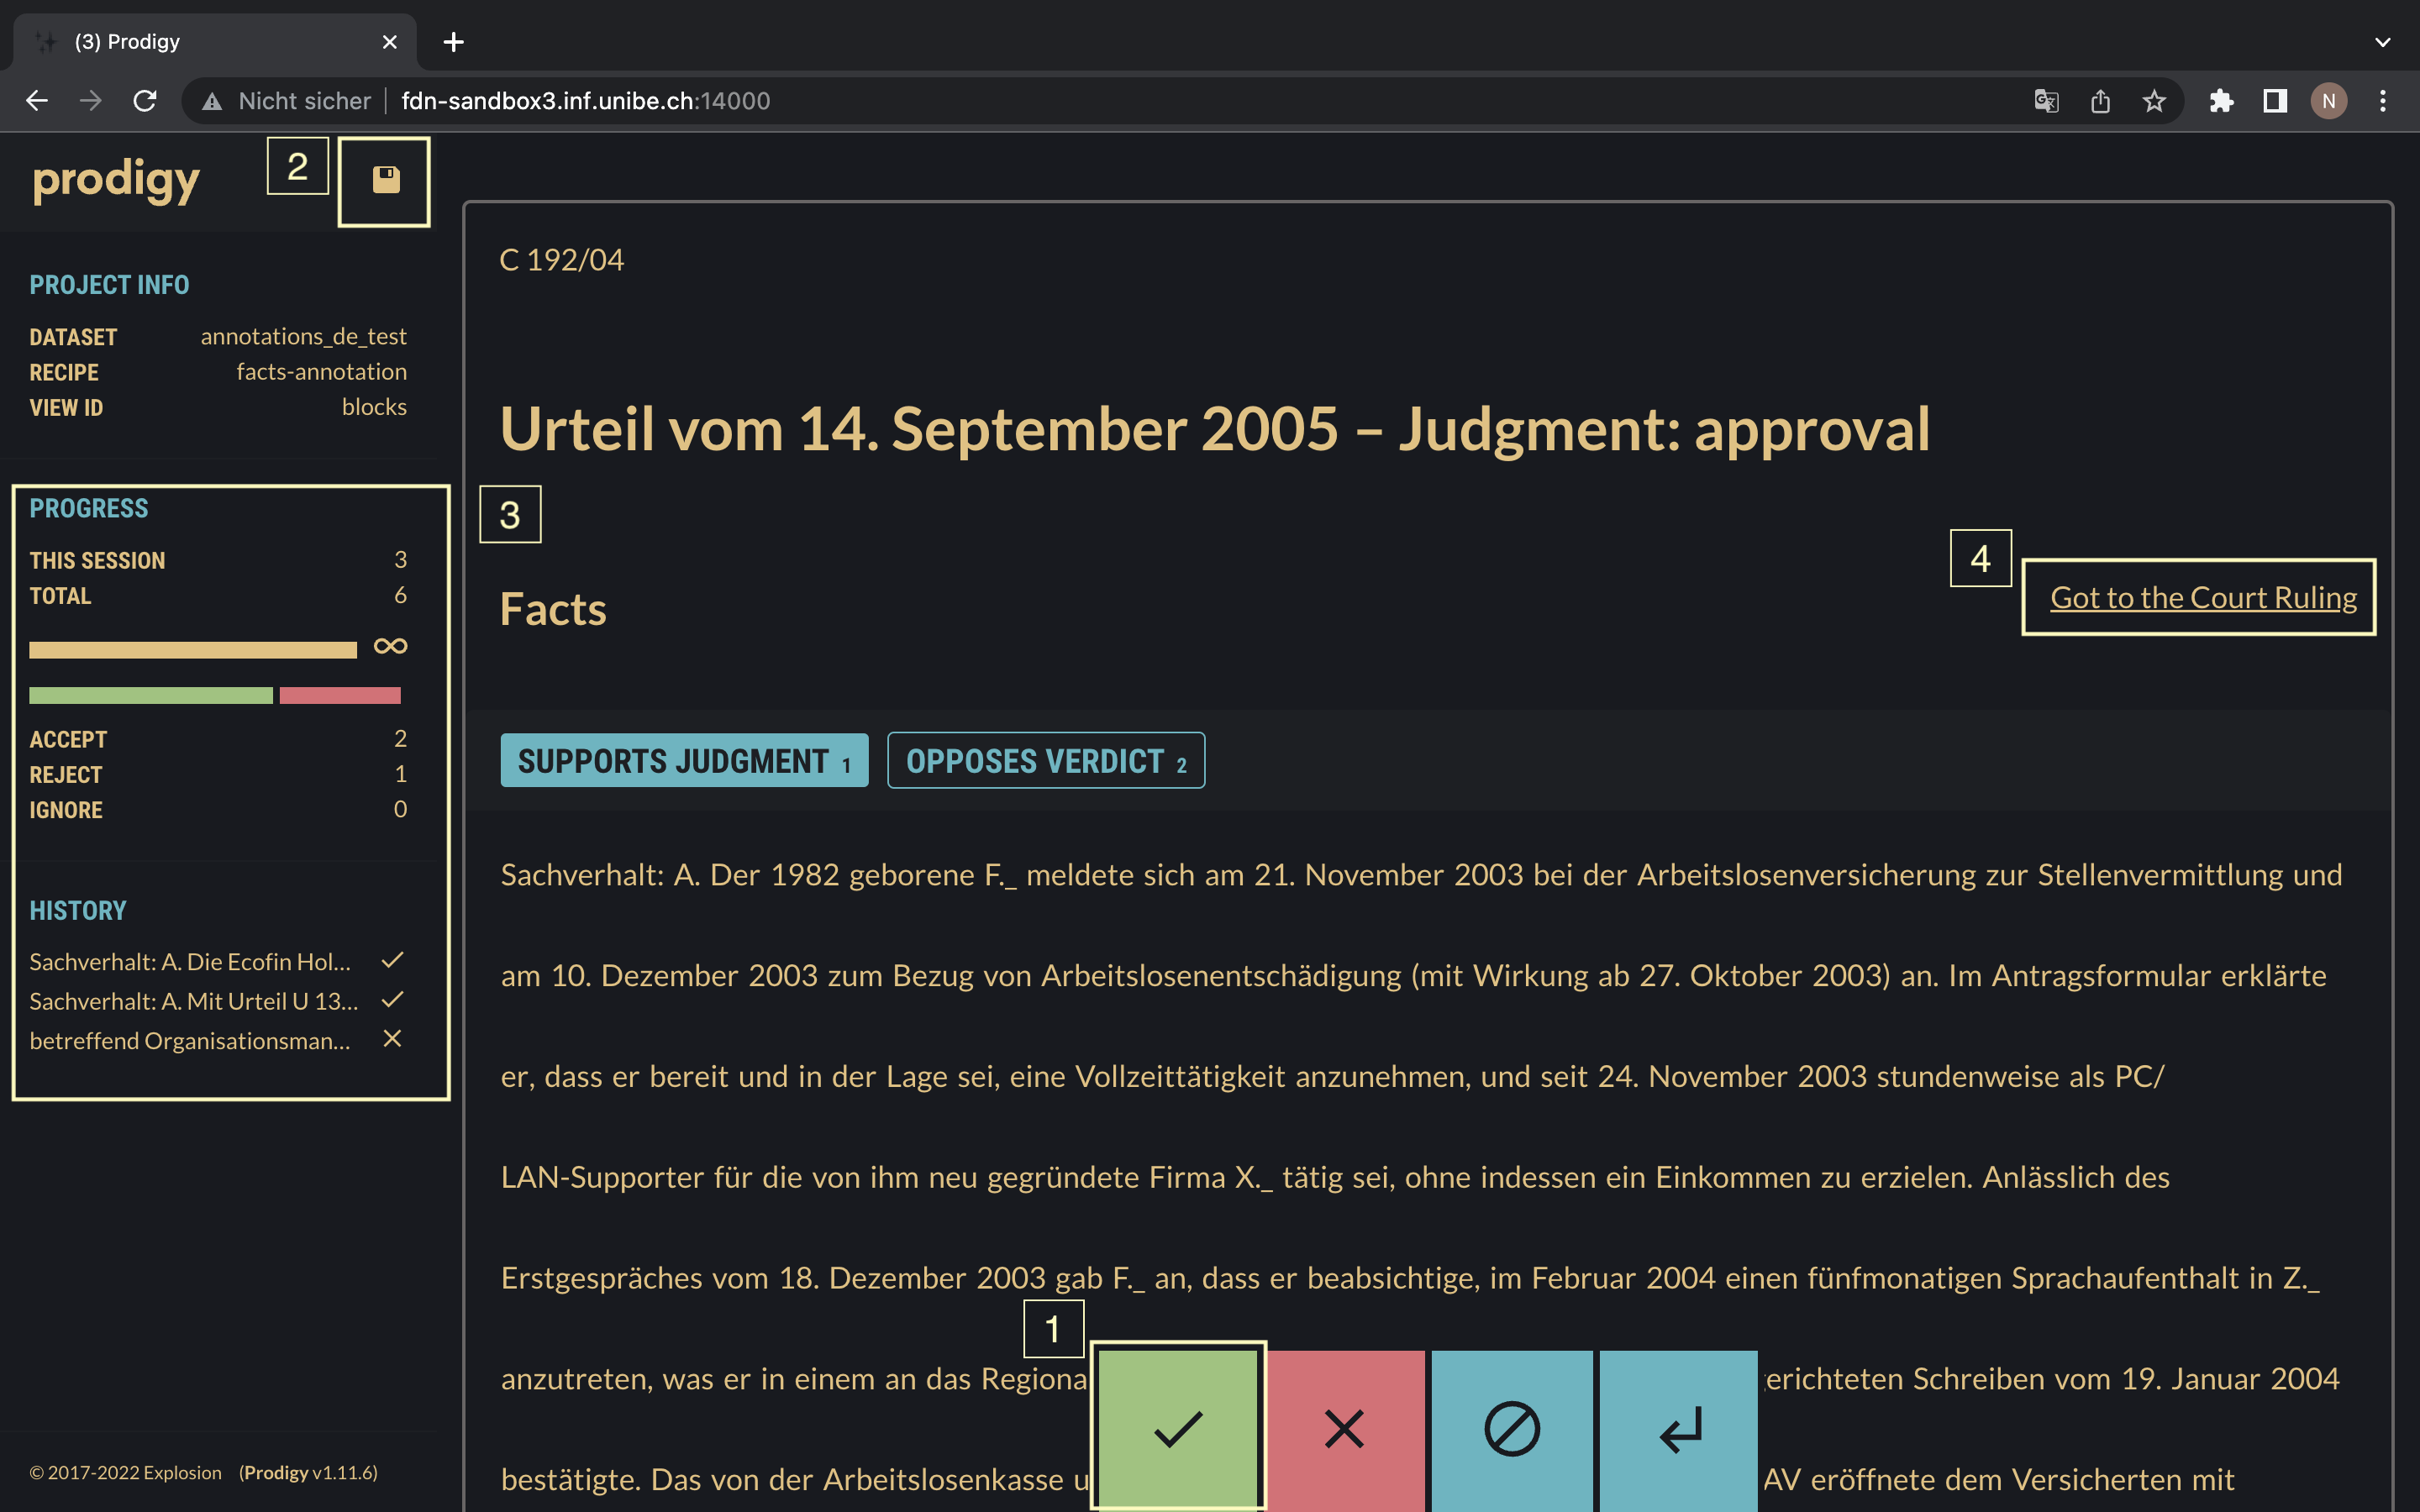
\includegraphics[width=\textwidth]{overview}}
     \caption{Screenshot of the case overview on prodigy}
     \label{overview}
\end{figure}
\pagebreak


\subsection{Reject or Ignore a Case}
\label{reject-ignore-case}
To reject a case state your reasoning in the comment section and press the red cross to reject it. To ignore it, press the blue button with the stop signal after commenting. Do not forget to save your progress. Figure \ref{reject_ignore} shows the interface of the comment section and the ignore and reject buttons. 

\begin{figure}[h]
    \makebox[\textwidth]{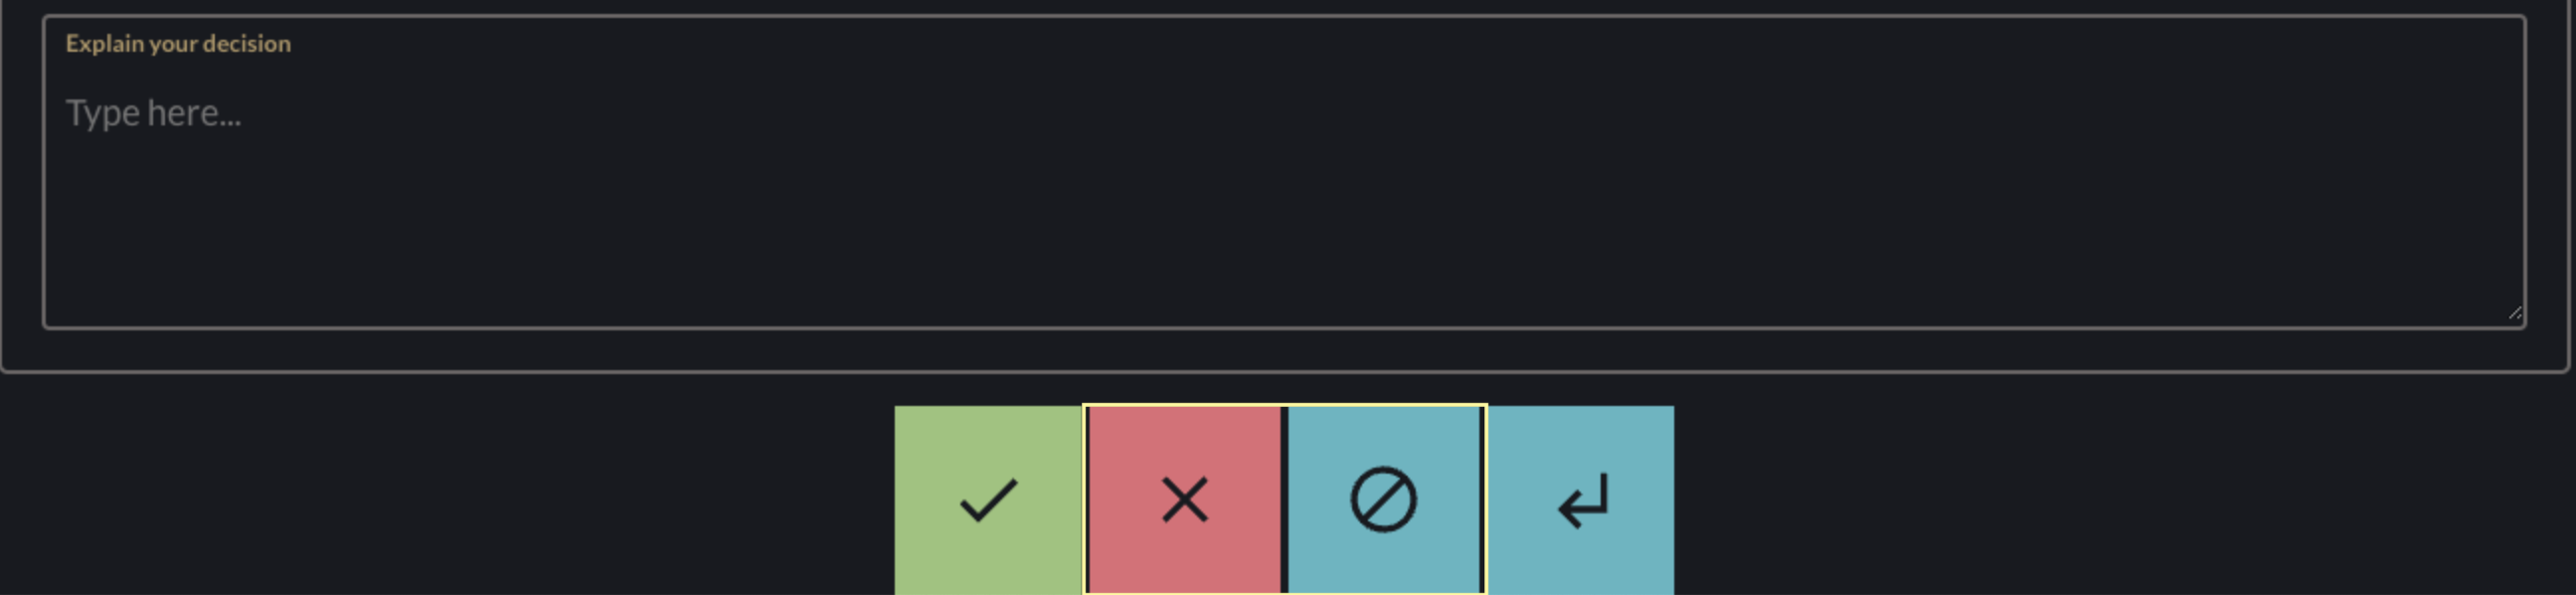
\includegraphics[width=\textwidth]{Bachelorthesis/Annotationguidelines/images/reject_ignore.png}}
     \caption{Reject and Ignore buttons}
     \label{reject_ignore}
\end{figure}

\section{Change Log}
This change log documents the progress of these guidelines. When adapting these guideline please also add a new entry to the changelog using the following structure
\begin{mdframed}[frametitle={Template}]
\emph{Date – Title of changes}
\begin{itemize}
	\item Which parts were changed in which iteration?
    \item Why was this part changed
\end{itemize}
\end{mdframed}
\begin{mdframed}[frametitle={Change log}]
\emph{10.04.2022 – Formal changes after first feedback}
\begin{itemize}
	\item Which parts were changed in which iteration? 
	\begin{itemize}
	    \item Changed E. Leitner reference to the published article.
	    \item Corrected some spelling errors.
	    \item Integrated the figures into the text of the guidelines.
	    \item Changed label "opposes verdict" to "opposes judgment"
	\end{itemize} 
    \item Why was this part changed
    
    With this first adaption of the guidelines we mainly worked on some formal errors to standardize the format and clarify the instruction (especially with integrating the figures into the text). The label was changed to make the annotation and their interpretation more consistent.

\end{itemize}
\emph{23.04.2022 – Changes to Prodigy setup and new label}
\begin{itemize}
	\item Which parts were changed in which iteration? 
	\begin{itemize}
	    \item Named multi-user sessions where added to the Prodigy setup, which changed the annotators URLs in this document.
	    \item The label lower court was added as a new annotation category and subsequently to the prodigy setup. Explanation how and when to use it were added to section 2 and 3.
	    \item Directions on how to skip already annotated cases were added. To section 4.2
	\end{itemize} 
    \item Why was this part changed
    
    The named multi-user session was a pending part of the prodigy setup, which is now resolved. The URLs of the annotators had to be adapted accordingly. After a meeting with the lawyer and annotator Thomas Lüthi, we decided on adding the new label "lower court", to highlight it as a separate entity additionally to the existing two labels. 
    Correct sessions where not yet implemented in the first setup of Prodigy used for some annotations, for this reason directions on how to skip a case a already annotated case were added.
    
\end{itemize}
\end{mdframed}

\bibliographystyle{johd}
\bibliography{bib}
\listoffigures


\end{document}